
\chapter{État de l'art sur la détection de communautés et les réseaux dynamiques}
\chaptermark{État de l'art}
\minitoc
\label{chap:etat_art}
Dans cette thèse, nous étudions deux axes de recherche orthogonaux qui sont liés aux graphes: la détection de communautés et les extensions temporelles des graphes.
Ceux-ci seront présentés dans les sections~\ref{sec:intro_communaute} et \ref{sec:intro_extension_temporelle} après que nous soyons revenus, dans l section~\ref{sec:def_graphe}, sur quelques définitions et notations utiles pour manipuler des graphes.

Le premier axe de recherche est la détection de structures dans les graphes et plus particulièrement de communautés.
Une communauté est une partie du graphe telle qu'il existe de nombreux liens à l'intérieur de la communauté et moins de liens entre cette communauté et le reste du graphe.
Cependant aucune définition ne fait l'unanimité.
La notion de communauté dépend du contexte et de la méthode.
Malgré cette définition floue, des structures communautaires ont été trouvées dans de nombreux graphes dans différents domaines tels que le réseau constitué des régions du cerveau \cite{DeReus2014}, un réseau de distribution d'eau \cite{DiNardo2015} et un réseau d'interactions d'animaux \cite{Farine2015}.
Ces notions de communautés et les méthodes de détection sont définies dans la section~\ref{sec:intro_communaute}.

Le second axe de recherche est la prise en compte du temps dans la théorie des graphes.
La première approche fut de complètement ignorer l'information temporelle et de considérer que tous les liens apparaissent en même temps; on parle alors de graphe agrégé.
Cependant, l'utilisation d'un graphe agrégé manque de pertinence, lorsque le réseau change trop au cours du temps~\cite{Holme2015b}.
Si tel est le cas, certaines structures présentes dans le graphe peuvent n'être que des artefacts de l'agrégation temporelle.
Imaginons par exemple un graphe représentant les alliances politiques dans un pays sur une longue période.
Si toutes les alliances politiques sont agrégées, alors les personnes changeant de parti politique seront faussement considérées comme influentes car connectées à plusieurs partis alors qu'elles peuvent, en réalité, ne plus avoir de contact dans leur ancien parti.
Ainsi, il n'est plus possible d'observer la répartition des alliances politiques dans ce genre de réseau si l'agrégation temporelle est trop importante~\cite{Mucha2010}.

Si l'on prend en compte le temps, alors il devient possible de détecter des structures plus fines que dans le cas statique.
En effet, on peut détecter des instants où l'organisation générale change~\cite{Rosvall2010}, comprendre quels sont les instants où un n\oe{}ud est important~\cite{Magnien2015,Costa2015,Takaguchi2016}, ou bien détecter des groupes temporels~\cite{Cazabet2010}.
Pour ce faire, plusieurs extensions de la théorie des graphes ont été proposées et elles sont présentées dans la section~\ref{sec:intro_extension_temporelle}.


\section{Définitions dans les graphes}
\label{sec:def_graphe}

Un graphe $G$ est défini par un couple $(V, E)$ où $V$ est un ensemble de n\oe{}uds et $E \subseteq V \times V$ est un ensemble de liens, chaque lien étant une paire de n\oe{}uds.
Sauf mention contraire, nous considérons des graphes non-orientés, c'est-à-dire pour toute paire de n\oe{}uds $u,v \in V$, les liens $(u,v)$ et $(v,u)$ sont équivalents.
Nous considérons également uniquement des liens non-pondérés, c'est-à-dire qu'un lien est soit présent soit absent.
Enfin, nous ne considérons que des graphes simples, c'est-à-dire qu'il n'existe au maximum qu'un seul lien entre deux n\oe{}uds et aucun lien de la forme $(u,u)$.
Ceci est en opposition avec les graphes multiples où il peut exister plusieurs liens entre deux n\oe{}uds.

Par convention, nous notons $n=|V|$ le nombre de n\oe{}uds et $m=|E|$ le nombre de liens.
On suppose en général que $V=\{1, ..., n\}$.
Il est possible de représenter un graphe $G$ par une matrice carrée $A$ de taille $n$ où l'élément $A_{i,j} \ \forall i,j \in V$ est égal à $1$ si un lien relie les n\oe{}uds $i$ et $j$ et $0$ sinon.
Avec ces notations, nous définissons les notions suivantes:
\begin{description}
\item[Degré] Le degré d'un n\oe{}ud $i$, noté $d_i$, est égal au nombre de liens reliés à $i$: $d_i = \sum_{j \in V} A_{i,j}$;
\item[Densité] La densité, $\delta(G)$ d'un graphe est la probabilité que deux n\oe{}uds pris au hasard soient reliés par un lien: $\delta(G)=\dfrac{2m}{n(n-1)}$;
\item[Degré moyen] Le degré moyen $\tilde{\delta}(G)$ est égal à : $\tilde{\delta}(G)=\dfrac{2m}{n}$;
\item[Chemin] Un chemin dans un graphe est une suite de liens $((u_1,v_1),...,(u_k,v_k))$ telle sorte $v_{i}=u_{i+1} \ \forall i \in [1,k-1]$;
\item[Cycle] Un cycle est un chemin dont les premier et dernier n\oe{}uds sont identiques;
\item[Graphe connexe] Un graphe est dit connexe s'il existe un chemin entre toutes les paires de n\oe{}uds du graphe;
\item[Composante connexe] Une composante connexe est un ensemble de n\oe{}uds $V'\subseteq V$ qui est connexe et maximal, c'est-à-dire qu'il n'est pas possible d'ajouter un n\oe{}ud dans $V'$ de telle sorte que $V'$ soit connexe;
\item[Arbre] Un arbre est un graphe connexe sans cycle; il contient $n-1$ liens pour $n$ n\oe{}uds;
\item[Clique] Une clique, aussi appelée graphe complet, est le graphe le plus dense et elle est composée de $\dfrac{n(n-1)}{2}$ liens pour $n$ n\oe{}uds;
\item[Sous-graphe] Un graphe $G'=(V',E')$ est un sous-graphe de $G$ si et seulement si $V' \subseteq V$ et $E' \subseteq E$;
\item[Graphe induit] Le graphe induit par un ensemble de n\oe{}uds $V' \subseteq V$ est défini par $V'$ et $E'= E \cap (V' \times V')$.
\end{description}



\subsection{Groupes, partitions et couvertures}
En plus des n\oe{}uds et des liens, nous manipulons également des ensembles de liens et des ensembles de n\oe{}uds.
Par convention, notons $X \subseteq V$ un ensemble de n\oe{}uds et $Y \subseteq E$ un ensemble de liens.
Nous listons les notations utilisées dans le tableau~\ref{tab:notation_groupe_noeuds}.


\begin{table}
  \centering
  \hspace*{-18.225pt}
    \begin{tabular}{|c|c|}
     \hline
    \rule[-1ex]{0pt}{4ex} Notation & Définition \\
  \hline
		\hline
		\rule[-1ex]{0pt}{4ex}$V(Y)=\{u,\ \exists (u,v) \in Y \}$ & n\oe{}uds induits par les liens de $Y$\\
		\hline
        \rule[-1ex]{0pt}{4ex}$n_X=|X|$ & nombre de n\oe{}uds dans $X$\\
        \hline
        \rule[-1ex]{0pt}{4ex} $l_{in}(X)=|E \cap (X \times X)|$ & nombre de liens entre les n\oe{}uds de $X$\\
        \hline
        \rule[-1ex]{0pt}{4ex} $l_{out}(X)=|E \cap (X \times V \setminus X)|$ & nombre de liens entre les n\oe{}uds de $X$ et de $V \setminus X$ \\
        \hline
        \rule[-1ex]{0pt}{4ex} $l(X)=l_{in}(X)+l_{out}(X)$ & nombre de liens reliés aux n\oe{}uds de $X$\\
        \hline
        \rule[-1ex]{0pt}{4ex} $d_{in}(u,X)=|\{(u,v) \in E,\ v \in X\}|$ & nombre de liens entre $u$ et $X$ \\
        \hline
        \rule[-1ex]{0pt}{4ex} $d_{in}(X)=\sum_{u \in X} d_{in}(u,X)=2l_{in}(X)$ & somme des degrés internes des n\oe{}uds dans $X$ \\
        \hline
        \rule[-1ex]{0pt}{4ex} $d_{out}(u,X)=|\{(u,v) \in E,\ v \in V \setminus X\}|$ & nombre de liens entre $u$ et $V \setminus X$ \\
        \hline
       \rule[-1ex]{0pt}{4ex}  $d_{out}(X)=\sum_{u \in X} d_{out}(u,X)=l_{out}(X)$ & somme des degrés externes des n\oe{}uds dans $X$ \\
        \hline
        \rule[-1ex]{0pt}{4ex}  $d(X)=d_{in}(X)+ d_{out}(X)$ & somme des degrés des n\oe{}uds dans $X$ \\
        \hline
    \end{tabular}
    \caption{Liste des notations utilisées pour un ensemble de n\oe{}uds $X$ et un ensemble de liens $Y$.}
         \label{tab:notation_groupe_noeuds}
\end{table}%


\paragraph{Partitions et couvertures}
Nous définissons ici les structures de partitions et de couvertures appliquées au cadre spécifique des graphes.
Une partition de n\oe{}uds, $\mathcal{V}$, est un ensemble d'ensembles de n\oe{}uds: $\mathcal{V}= \{V_1,..., V_k\}$ tel que $\forall i \in [1,k]\ V_i \subseteq V$ et tel que:
\begin{enumerate}
\item La partition \emph{recouvre} la totalité des n\oe{}uds: $\bigcup_{i} V_i = V$.
\item Les ensembles de n\oe{}uds sont disjoints: $V_i \cap V_j = \emptyset\ \forall i,j \in [1,k],\ i \neq j$.
\end{enumerate}
Afin de manipuler une partition, nous définissons $\mathcal{V}(u)=V_i$ si et seulement si $u \in V_i$.
\bigskip

Une couverture est une extension des partitions car elle relâche la contrainte sur l'intersection.
Ainsi, une couverture de n\oe{}uds, $\mathcal{V}$, est aussi un ensemble d'ensembles de n\oe{}uds.
L'union des ensembles doit également être égal à $V$ mais en revanche deux ensembles de n\oe{}uds peuvent partager des n\oe{}uds: $\forall i,j \in [1,k], |V_i \cap V_j\ \geq 0$.
Une couverture est parfois aussi appelée partition chevauchante.

Nous avons détaillé les notions de partitions et couvertures de n\oe{}uds mais les mêmes définitions valent pour les partitions et couvertures de liens.
Enfin, il existe d'autres structures possibles, comme les structures non-exhaustives pour lesquelles un élément peut n'appartenir à aucun ensemble.

\subsection{Comparaison de partitions et couvertures}
Il est souvent utile de pouvoir comparer deux partitions ou deux couvertures entre elles.
Le but est de calculer une similarité entre deux structures de telle sorte que la similarité soit égal à $1$ si les deux structures sont identiques et qu'elle soit égal à $0$ ou $-1$ si elles sont complètement différentes.
Il existe pour ce faire des méthodes tirant parti de la structure d'ensembles et d'autres provenant de la théorie de l'information.

\paragraph{Approches ensemblistes}
\label{def:graphe_comparaison}
Il est possible de comparer deux ensembles $X$ et $Y$ en utilisant l'indice de Jaccard, $\mathbb{J}(X,Y) = \dfrac{|X \cap Y|}{|X \cup Y|}$, ou le \emph{F1 score}, $F_1(X,Y) = 2\dfrac{|X \cap Y|}{|X| + |Y|}$.
Avec l'indice de Jaccard ou le \emph{F1 score}, il est possible de mesurer la similarité entre deux partitions $\mathcal{X}$ et $\mathcal{Y}$:
\begin{equation}
sim(\mathcal{X},\mathcal{Y})=\frac{1}{|\mathcal{X}|}\sum_{X \in \mathcal{X}}\max_{Y\in \mathcal{Y}}\mathbb{J}(X,Y).
\end{equation}

Avec cette formulation, la similarité n'est pas symétrique.
C'est pourquoi la formule suivante lui est souvent préférée:

\begin{equation}
sim_{moy}(\mathcal{X},\mathcal{Y}) = \dfrac{sim(\mathcal{X},\mathcal{Y})+sim(\mathcal{Y},\mathcal{X})}{2}\,.
\end{equation}
Il existe d'autres méthodes pour symétriser la similarité, \emph{e.g.} la moyenne harmonique.
Cette méthode peut s'appliquer indifféremment aux partitions et aux couvertures.

On peut également utiliser le \emph{Rand Index}~\cite{Rand1971} qui lui ne s'applique qu'aux partitions.
Il mesure le nombre de paires de n\oe{}uds qui sont classées de la même manière dans les deux partitions; c'est à dire pour deux n\oe{}uds $u$ et $v$ soit $\mathcal{X}(u)=\mathcal{X}(v)$ et $\mathcal{Y}(u)=\mathcal{Y}(v)$ soit $\mathcal{X}(u)\neq \mathcal{X}(v)$ et $\mathcal{Y}(u)\neq \mathcal{Y}(v)$.
Plus formellement, soient
\begin{itemize}
\item $a_{11}$ le nombre de paires de n\oe{}uds de telle sorte qu'ils soient dans le même ensemble dans les deux partitions;
\item $a_{00}$ le nombre de paires de n\oe{}uds de telle sorte qu'ils soient dans des ensembles différents dans les deux partitions;
\item $a_{10}$ (resp. $a_{01}$) le nombre de paires de n\oe{}uds de telle sorte qu'ils soient dans le même ensemble dans $\mathcal{X}$(resp. $\mathcal{Y}$) et dans deux ensembles différents dans $\mathcal{Y}$ (resp. $\mathcal{X}$).
\end{itemize}
Avec ces notations, le \emph{Rand Index} est défini de la manière suivante:

\begin{equation}
RI(\mathcal{X},\mathcal{Y}) = \dfrac{a_{11} + a_{00}}{a_{11}+a_{01}+a_{10}+ a_{00}}
\end{equation}
Cependant, $a_{00}$ est souvent très grand comparé à $a_{11}$ car il est courant de ne pas mettre deux n\oe{}uds dans la même communauté.
\`A cause de cela, le \emph{Rand Index} peut être proche de $1$ même pour des partitions assez différentes.
Pour remédier à ce problème, le \emph{Adjusted Rand Index} (ARI)~\cite{Hubert1985} a été proposé .
Le \emph{Rand Index} et sa version ajustée permettent de comparer des partitions.
Porumbel \emph{et al.}~\cite{Porumbel2011} ont proposé l'Omega Index qui est une extension de l'ARI pour les couvertures.

\paragraph{Approche venant de la théorie de l'information}
On peut considérer que l'assignation d'un élément à un ensemble est une variable aléatoire.
Dans ce cas, la probabilité qu'un élément a d'être dans un ensemble $X \in \mathcal{X}$ est $P(X)= n_X/|V|$.
De manière similaire, la probabilité jointe est $P(X,Y) = |X \cap Y|/|V|$.
Avec ces définitions, il est possible de calculer l'entropie d'une partition, $H(\mathcal{X})$, l'entropie conditionnelle, $H(\mathcal{X}|\mathcal{Y})$ et l'information mutuelle $I(\mathcal{X},\mathcal{Y})$.
Cette dernière est définie par $I(\mathcal{X}, \mathcal{Y}) = H(\mathcal{X}) - H(\mathcal{X}|\mathcal{Y})$.
L'entropie, $H(\mathcal{X})$, et l'entropie conditionnelle, $H(\mathcal{X}|\mathcal{Y})$, sont, selon la définition de Shanon: 
\begin{equation}
H(\mathcal{X}) = - \sum_{X \in \mathcal{X}} P(X)\log(P(X)),\quad H(\mathcal{X}|\mathcal{Y}) = -\sum_{X \in \mathcal{X},\ Y \in \mathcal{Y}} P(X, Y) \log \dfrac{P(X,Y)}{P(Y)}.
\end{equation}
Afin de normaliser l'information mutuelle, Danon \emph{et al.}~\cite{Danon2005a} ont défini l'information mutuelle normalisée (NMI$_{shanon}$):
\begin{equation}
 NMI_{shanon}(\mathcal{X},\mathcal{Y}) = \dfrac{2I(\mathcal{X},\mathcal{Y})}{H(\mathcal{X})+H(\mathcal{Y})}.
\end{equation}

Lancichinetti et Fortunato l'ont par la suite étendue pour prendre en compte les couvertures~\cite{Lancichinetti2009d}.
Le choix de la normalisation dans le cas chevauchant est cependant toujours ouvert~\cite{McDaid2011,Zhang2015c}.

\resume{
Il est intéressant de noter que la littérature sur la comparaison de partitions et de couvertures est assez restreinte comparée à celle sur la détection de communautés (présentée ci-après).
En effet, il semble qu'uniquement 3 similarités soient couramment utilisées: la similarité se basant sur l'indice de Jaccard, l'Omega Index et la NMI.
Tous les indices de similarité ont été étendus aux couvertures de manière assez convaincante.
Il est également important de noter l'existence d'implémentations librement accessibles de la majeure partie de ces métriques\, \footnote{\url{https://github.com/aaronmcdaid/Overlapping-NMI}}\,\footnote{\url{http://scikit-learn.org/stable/modules/clustering.html\#clustering-evaluation}}.
}


\section{Communautés dans les graphes}
\label{sec:intro_communaute}

La détection de communautés dans les graphes est un très vaste champ de recherche et il serait illusoire de prétendre énumérer les méthodes existantes dans ce domaine: elles sont extrêmement nombreuses.
Aussi les critères permettant la caractérisation d'une communauté peuvent varier selon le contexte~\cite{Leskovec2008,Coscia2011,Yang2015,Jeub2015}.
Ces méthodes sont tout de même réparties en plusieurs catégories selon qu'elles capturent une partition ou une couverture de n\oe{}uds.
Ces deux structures correspondent à deux visions possibles de l'organisation d'un graphe et du réseau sous-jacent.
Nous présentons ces deux catégories dans les sous-sections suivantes.
Il en existe également une troisième qui est la détection de communautés sous la forme de partitions de liens que nous traitons dans le chapitre~\ref{chap:Expected_Node}\,\footnote{La détection de couvertures de liens est encore très peu étudié.}.

\subsection{Partitions de n\oe{}uds}
\label{subsec:Part_noeuds}
Afin de mieux comprendre ce que peut capturer une partition de n\oe{}uds, il est plus facile de s'appuyer sur un exemple.
Dans l'étude de Stehlé \emph{et al.}~\cite{Stehle2011}, des enfants d'une école primaire ont porté pendant $2$ jours des capteurs enregistrant lorsque deux enfants sont à une distance de moins de 1 mètre 50.
Ce dispositif permet de mesurer les interactions entre élèves et de construire le graphe des relations à l'école.
Un lien existe entre deux élèves s'ils ont interagi au moins une fois ensemble.
Une illustration du graphe obtenu est visible dans la figure~\ref{fig:ecole_primaire}.
La classe de chaque élève est également connue.
Comme chaque élève appartient à une et une seule classe, les classes forment une partition des élèves.
Cette partition est une bonne structure communautaire car on remarque que les élèves d'une même classe interagissent beaucoup entre eux mais peu avec les élèves des autres classes.
Cela se remarque bien pour la classe $3A$.
Il existe beaucoup de liens entre les élèves de la classe $3A$ mais aucun avec les élèves de la classe $5A$ par exemple.
En cela, la structure en classes constitue une vérité de terrain.

\begin{figure}
\centering
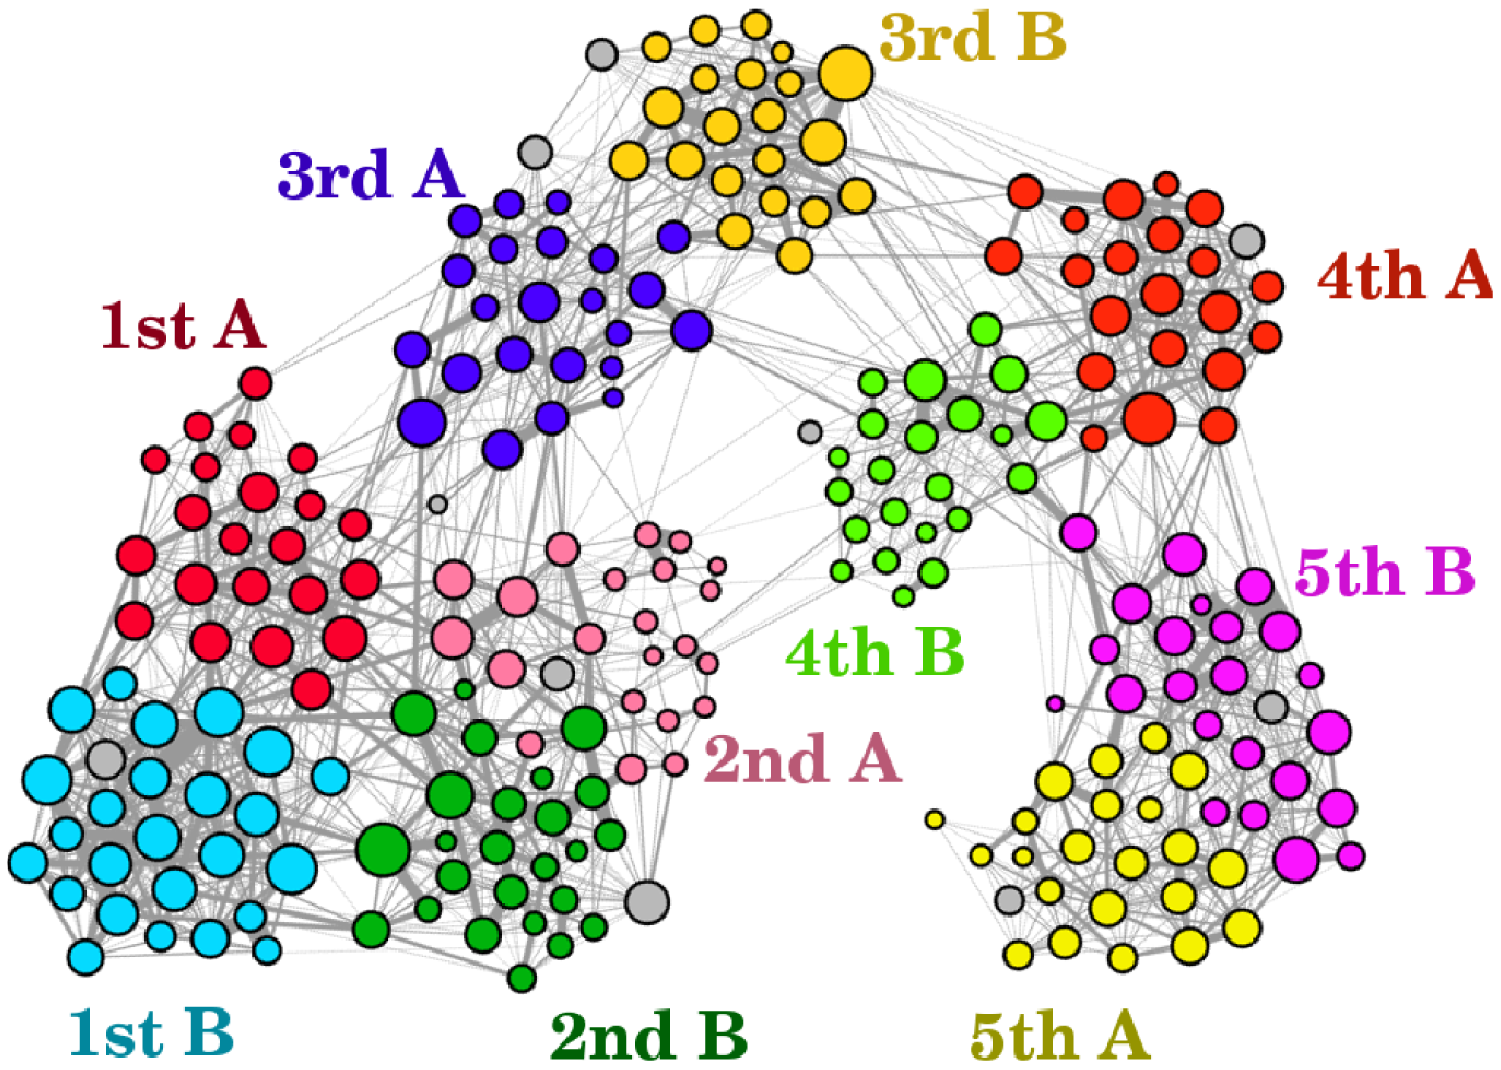
\includegraphics[width=0.7\linewidth]{img/Intro/ecole_primaire}
\caption{Graphe de contact des enfants d'une école primaire. L'épaisseur du lien représente la durée d'interaction entre deux élèves. La couleur représente la classe de chaque élève et la taille représente le degré du n\oe{}ud. Les professeurs sont en gris.\protect\footnotemark}
\label{fig:ecole_primaire}
\end{figure}
\footnotetext{Image provenant de \url{http://journals.plos.org/plosone/article?id=10.1371/journal.pone.0023176}.}

Afin de capturer des partitions de n\oe{}uds, beaucoup de méthodes existent.
Des états de l'art sont d'ailleurs régulièrement publiés~\cite{Fortunato2010,Plantie2013a, Malliaros2013a, Harenberg2014a}.
Afin de faciliter la compréhension du sujet, nous détaillons ici quelques unes des méthodes les plus utilisées.

\subsubsection{Méthodes utilisant un modèle}
\label{def:Modularite}
Une communauté étant souvent définie comme devant être très densément connectée, le problème est de trouver une fonction capable d'évaluer la qualité d'une communauté.
Pour ce faire, il faut définir une métrique qui mesure la densité, \emph{e.g.} le nombre de liens dans un groupe.
Puis, il est nécessaire de définir comment évaluer cette métrique.

Il est possible d'utiliser une métrique en la normalisant par ses bornes minimum et maximum.
Avec une métrique normalisée entre $0$ et $1$, un groupe est alors considéré comme très connecté si son évaluation est supérieure à un certain seuil.
Par exemple, le nombre de liens entre $n$ n\oe{}uds peut être normalisé par le nombre de liens dans un arbre et dans une clique de taille $n$. 
Cette approche n'est cependant pas adaptée pour la recherche de communautés car elle ne tient pas compte de la structure globale du graphe\,\footnote{Cette approche est plus appropriée dans la recherche des groupes les plus denses~\cite{Balalau2015}.}.
Prenons l'exemple du graphe constitué d'une unique clique.
Dans ce graphe, tout groupe de n\oe{}uds est également une clique et par conséquent tout groupe de n\oe{}uds a une évaluation parfaite de $1$.
Chaque groupe serait donc une très bonne communauté selon cette évaluation.
Or, le graphe constitué d'une unique clique ne possède pas de structure communautaire contrairement au graphe dans la figure~\ref{fig:ecole_primaire}.
Il est donc nécessaire de trouver une autre approche.

\bigskip

Plutôt que de normaliser une métrique par ses valeurs minimale et maximale, il est intéressant de considérer l'écart à une valeur attendue.
L'idée est la suivante: quelle serait la valeur attendue de la métrique considérée si le graphe n'avait pas de structure communautaire?
Le problème est alors de "retirer" la structure communautaire du graphe ou bien de définir un ensemble de graphes similaires au graphe initial mais n'ayant pas de structure communautaire.
Ce processus définit alors ce qu'on appelle un \emph{modèle nul}.
Détecter des communautés revient alors à trouver des groupes qui s'éloignent du modèle nul pour lequel il n'existe pas de communauté.

Ce changement est astucieux car il est relativement aisé de définir des graphes n'ayant pas de structure.
Il suffit de créer des graphes complètement aléatoires~\cite{Erdos1959} dont les liens sont tirés de manière uniforme.
Afin que les graphes aléatoires puissent être comparés au graphe initial, des contraintes sont généralement ajoutées et donnent lieu à différents modèles nuls.
Le premier modèle nul de graphe est celui de Erdös-Rényi~\cite{Erdos1959} dans lequel le nombre de liens et le nombre de n\oe{}uds des graphes aléatoires doivent être les mêmes que dans le graphe initial.
Un autre modèle très couramment utilisé est le modèle de configuration~\cite{Bender1978a}.
Dans ce modèle, la distribution des degrés est également fixe.
Le modèle de configuration est privilégié car il a été observé que les graphes provenant de données réelles ont une distribution des degrés très éloignée d'une distribution uniforme.
C'est pourquoi l'ajout de la contrainte sur les degrés permet de considérer des graphes plus proches du graphe initial. 
Il existe d'autres modèles possibles considérant d'autres contraintes, notamment sur le nombre de cliques de taille 3 (nommées triangles en théorie des graphes)~\cite{Newman2009}.

\paragraph{Modularité}
La modularité~\cite{Newman2004} est une fonction qui associe à chaque partition de n\oe{}uds une valeur entre $-1$ et $1$.
Plus la valeur de modularité d'une partition est élevée, plus la partition est censée détecter une bonne structure communautaire.
La modularité est définie de la manière suivante pour une partition $\mathcal{C}$:

\begin{equation}
Q(\mathcal{C}) = \dfrac{1}{2m}\sum_{i,j \in V} \left(A_{ij} - \dfrac{d_id_j}{2m}\right)\ \delta_{\mathcal{C}(i)=\mathcal{C}(j)} \ ,
\end{equation}
où $\delta_{C(i)=C(j)}$ est égal à $1$ si $i$ et $j$ sont dans la même communauté et $0$ sinon.
Il s'agit pour deux n\oe{}uds d'une même communauté de comparer la présence ou l'absence d'un lien, $A_{ij}$, à la probabilité que ces n\oe{}uds soient reliés dans le modèle de configuration, $\dfrac{d_id_j}{2m}$.
L'idée sous-jacente est que les n\oe{}uds d'une communauté devraient partager plus de liens que ce qui est attendu dans le modèle de configuration.
De très nombreux travaux ont étudié les caractéristiques de la modularité et son optimisation.
Tout d'abord, il a été montré que l'optimisation de la modularité est un problème NP-Complet~\cite{Brandes2007}.
Il est donc nécessaire de recourir à des heuristiques\,\footnote{Une heuristique est une méthode de calcul qui fournit rapidement (en temps polynomial) une solution réalisable, pas nécessairement optimale, pour un problème d'optimisation.} afin de trouver rapidement une partition proche de l'optimum.
Parmi l'ensemble des algorithmes existants, l'algorithme de Louvain~\cite{Blondel2008a} est l'un des plus rapide.
Il existe également des variantes de cet algorithme~\cite{Huang2015,Traag2015c}.

D'autres travaux se sont attachés à l'étude de la modularité.
Il a été montré que la modularité souffre du problème de limite de résolution~\cite{Fortunato2007,Lancichinetti2011}: il n'est pas possible de détecter de petites communautés lorsque le graphe est grand.
Cela est dû au modèle de configuration qui présuppose une répartition uniforme des tailles des communautés.
Il a par ailleurs été montré que la modularité n'offre pas de maximum clair et que beaucoup de partitions différentes ont des évaluations proches~\cite{Good2010}.
Pour répondre à ces problèmes, il existe différentes variantes de la modularité~\cite{Reichardt2006,Delvenne2010}.

%\paragraph{Surprise}
%La fonction Surprise~\cite{Aldecoa2011,Traag2015b} est une autre fonction de qualité qui se base quant à elle sur le modèle de Erdös-Rényi pour évaluer la surprise d'observer un groupe de n\oe{}uds relié par $l$ liens.

\paragraph{\emph{Stochastic Block Model}}
Nous avons défini précédemment la notion de modèle nul permettant de comparer une structure d'un graphe à l'absence de communautés.
Il est également possible d'utiliser un modèle génératif modélisant une structure communautaire puis de vérifier \emph{a posteriori} si ce modèle pourrait être à l'origine du graphe observé.
Le problème de détection de communauté est alors un problème d'inférence qui est traité avec des outils statistiques tel que le \emph{stochastic block model} (SBM)~\cite{Holland1983a,Nowicki2001}.
L'idée derrière le SBM est la suivante: la probabilité que deux n\oe{}uds soient reliés dépend uniquement de leur groupe respectif.
Si le graphe a une structure communautaire\,\footnote{Le SBM permet également de représenter d'autres type de structures.}, alors deux n\oe{}uds d'une même communauté devraient avoir une forte probabilité d'être connectés.
\`A l'inverse, deux n\oe{}uds de deux communautés différentes devraient avoir une probabilité assez faible d'être connectés.
Le SBM est défini par de nombreux paramètres: le nombre de groupes, l'assignation d'un groupe à chaque n\oe{}ud et les probabilités d'interactions entre les groupes.
Avec un jeu de paramètres donné, il est possible de calculer la vraisemblance que ce jeu de paramètres soit à l'origine du graphe.
Trouver une partition de n\oe{}uds dans ce contexte est alors équivalent à trouver le jeu de paramètres qui est le plus vraisemblablement à l'origine du graphe.


Dans le SBM, tous les n\oe{}uds sont considérés comme équivalents en particulier vis-à-vis du degré, ce qui peu courant avec des graphes provenant de données réelles.
C'est pourquoi une version tenant compte du degré des n\oe{}uds a été proposée: le Degree-corrected Stochastic Block Model (DSBM)~\cite{Karrer2011}.
Enfin d'après des récents travaux~\cite{Newman2016}, il semblerait qu'optimiser la vraisemblance du DSBM et la modularité soient des problèmes équivalents.

\subsubsection{Méthodes utilisant des marches aléatoires}
Il existe d'autres approches que celles basées sur un modèle nul ou sur un modèle génératif.
Il y a notamment les méthodes utilisant les marches aléatoires \cite{Pons2005,Rosvall2008}.
Ces méthodes partent de l'observation qu'un marcheur aléatoire reste longtemps dans une communauté densément connectée.

En particulier, la méthode Infomap~\cite{Rosvall2008} repose sur l'idée très élégante est suivante:
une partition de n\oe{}uds est une carte du graphe et, en ce sens, elle doit aider sa lecture.
Une carte est efficace si elle permet de mieux comprendre l'objet d'étude, c'est à dire si elle réduit sa complexité.
Considérons la carte de France, les départements découpent l'espace en zones disjointes et la majorité des routes sont à l'intérieur des départements.
Aussi, il est courant qu'un nom de ville soit unique dans un département mais qu'il puisse être utilisé dans plusieurs départements.
De plus, un voyageur se déplaçant aléatoirement sur les routes a peu de chance de sortir d'un département dans un temps donnée.
Pour décrire, \emph{a posteriori}, l'ensemble des villes traversées par ce voyageur, il suffit alors de donner le département initial puis la liste des villes visitées.
Il n'est pas nécessaire de répéter le département pour chaque ville si le voyageur n'en est pas sorti.
En ce sens, la découpe d'un pays en départements permet de réduire la complexité de la description du voyage.
Il s'agit donc d'un problème lié à la théorie de l'information et de sa compression.
De manière similaire, Rosvall et Bergstrom utilisent des marcheurs aléatoires se déplaçant sur les n\oe{}uds du graphe et les communautés comme zones du graphe.
Si les communautés sont bien formées, alors les marcheurs aléatoires restent bloqués à l'intérieur des communautés et la description de leur marche est courte.
La longueur de cette description devient alors la signature de la partition et plus la signature est courte, meilleure la partition est.

Le phénomène de limite de résolution a également été étudié dans le cadre de Infomap~\cite{Kawamoto2015} mais il est beaucoup moins prononcé.

\paragraph{Autres méthodes}
Il existe bien d'autres méthodes pour détecter des communautés en tant que partition des n\oe{}uds.
Les méthodes spectrales~\cite{Donetti2004,Mitrovic2009} se basent sur les vecteurs propres de la représentation d'un graphe sous la forme d'une matrice.
De manière moins formelle, il existe également les méthodes de \emph{Label Propagation Algorithm} (LPA)~\cite{Raghavan2007a,Li2014c}.
Dans ces méthodes, chaque n\oe{}ud a initialement un label puis à chaque itération chaque n\oe{}ud prend comme label l'un des labels de ses voisins.
En général, un n\oe{}ud prend comme label celui qui est le plus représenté parmi ses voisins.
Au bout d'un certain nombre d'itérations ou une fois à l'équilibre, il ne reste que quelques labels dans le graphe et ils représentent les communautés.


\resume{Il existe de très nombreuses méthodes pour la détection de communautés en tant que partition de n\oe{}uds. Il semble que les méthodes d'optimisation de \textbf{modularité}, la méthode \textbf{Infomap} et les \textbf{Stochastic Block Model} soient les plus utilisées dans la littérature.}

\subsection{Couverture de n\oe{}uds}
\label{subsec:cover}
Jusqu'à maintenant, nous avons considéré les communautés comme des partitions de n\oe{}uds.
Or, les partitions sont très restrictives et ne peuvent pas représenter toutes les situations possibles.
Prenons l'exemple d'un graphe reflétant des interactions entre personnes.
Il existe des communautés qui sont disjointes comme le travail et la famille mais bien souvent des personnes appartiennent à plusieurs groupes, voir l'exemple dans la figure~\ref{fig:ex_overlap_communaute}.
Ainsi le groupe des personnes faisant du sport et le groupe des personnes travaillant ensemble peuvent ne pas être disjoints.
Si tel est le cas, alors il n'est plus possible de représenter ces communautés avec une partition.
Il est nécessaire de manipuler une couverture de n\oe{}uds.
Ainsi dans l'exemple de la figure~\ref{fig:ex_overlap_communaute}, les n\oe{}uds rouges appartiennent à deux groupes au lieu d'un seul.

\begin{figure}
	\centering
	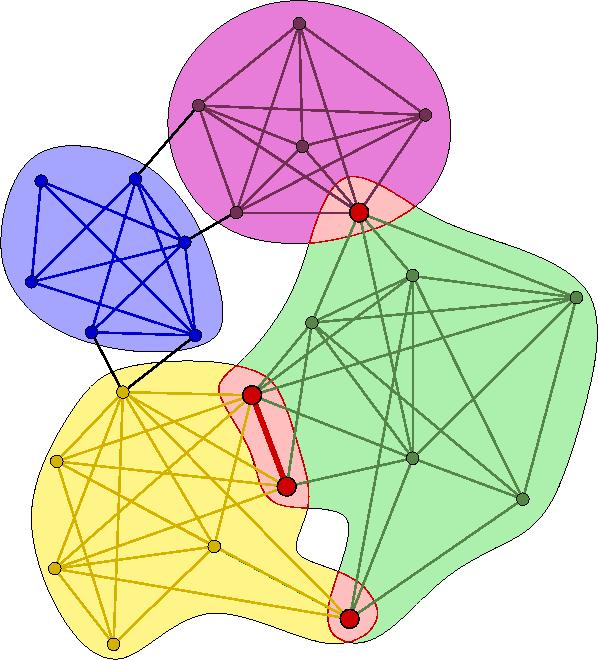
\includegraphics[width=0.31\linewidth]{img/Intro/Illustration_of_overlapping_communities.jpg}
	\caption{Exemple de graphe avec une structure communautaire chevauchante représentée par les couleurs\,\protect\footnotemark.}
	\label{fig:ex_overlap_communaute}
\end{figure}
\footnotetext{Image provenant de \url{https://en.wikipedia.org/wiki/Clique_percolation_method}.}

Une fois encore, la littérature est très vaste dans ce domaine et nous ne ferons pas une liste exhaustive des méthodes existantes.
Il existe de nombreux états de l'art dans le domaine~\cite{ Kanawati2014, Xie2013,Bandyopadhyay2015, Hric2014a}.

Une des plus anciennes méthodes de détection de couverture de n\oe{}uds est la \emph{Clique Percolation Method} (CPM)~\cite{Palla2005}.
L'algorithme CPM repose sur le principe de transitivité qui serait à l'origine des communautés: si $i$ et $j$ sont reliés par un lien, alors un n\oe{}ud $k$ qui serait relié à $i$ aurait une forte chance d'être également connecté à $j$.
Il s'agit de la formalisation du proverbe "Les amis de mes amis sont aussi mes amis".
Si ce principe est réellement à l'origine des communautés, alors les communautés doivent être composées de plusieurs cliques.
C'est pourquoi CPM cherche l'ensemble des cliques d'une taille $k$ donnée\,\footnote{En général, $k$ est compris entre 3 et 5 pour des raisons de coût de calcul.} puis fusionne toutes les cliques qui partagent suffisamment de n\oe{}uds, en général $k-1$. 
Comme cette méthode est relativement coûteuse en temps de calcul, Kumpula \emph{et al.}~\cite{Kumpula2008} ont repris le même mécanisme en optimisant le mode de calcul.

\subsubsection{Extensions des méthodes de détection de partitions}

La majorité des méthodes existantes pour les partitions ont été adaptées pour manipuler les couvertures de n\oe{}uds.
Il existe notamment plusieurs extensions de la modularité~\cite{Shen2009,Nicosia2009}.
Cependant ces extensions ne reposent plus sur un modèle nul car elles introduisent des termes de normalisation.
Par conséquent, ces extensions sont beaucoup moins utilisées que la modularité initiale.

\paragraph{Stochastic Block Model}
En revanche, le SBM s'adapte très bien aux couvertures de n\oe{}uds.
Une extension du SBM est le \emph{Mix-Membership Stochastic Block Model} (MMSBM)~\cite{Airoldi2008} qui permet à un n\oe{}ud d'être assigné plusieurs groupes.
Dans~\cite{Gopalan2013a}, les auteurs utilisent la même méthode mais en échantillonnant le graphe initial afin de réduire le coût de calcul.
Il existe d'autres méthodes utilisant des modèles génératifs~\cite{Ball2011,Yang2013}.
Ces méthodes se basent sur des graphes d'affiliation~\cite{BreigerRonald1974}.
Un graphe d'affiliation est un graphe biparti entre les n\oe{}uds d'une part et les communautés d'autre part.
Dans la méthode de Ball \emph{et al.}~\cite{Ball2011}, ce graphe d'affiliation est pondéré et la pondération représente la propension d'un n\oe{}ud à créer des liens dans un groupe donné tandis que pour Yang et Leskovec~\cite{Yang2013}, il s'agit du facteur d'appartenance du n\oe{}ud au groupe.
Une fois le graphe d'affiliation défini, il est nécessaire de savoir recréer la matrice d'adjacence et, en ce sens, ces méthodes se rapprochent des méthodes de factorisation en matrices non-négatives~\cite{Lee1999}.
Le but de la factorisation non-négative d'une matrice donnée est de trouver deux matrices dont les valeurs sont non-négatives telles que leur combinaison permette de retrouver la matrice initiale.

Jusqu'à récemment ce genre de technique généralisant le SBM ne pouvait s'appliquer qu'à des graphes relativement petits.
Cependant, de nouvelles méthodes~\cite{Gopalan2013a, Yang2013} arrivent à traiter des graphes ayant énormément de liens, de l'ordre $10^{9}$ à $10^{12}$ liens.



\paragraph{Propagation de label}
Des méthodes ont étendu la propagation de label aux couvertures de n\oe{}uds~\cite{Gregory2010,Xie2011}.
Le principal changement est qu'un n\oe{}ud ne stocke plus un unique label mais soit plusieurs labels, soit des fréquences d'apparition de labels.
Ainsi à la fin de l'algorithme, les communautés d'un n\oe{}ud sont les labels les plus fréquents.
Cependant, ce mécanisme de propagation change radicalement l'idée initiale.
En effet, la diffusion d'un label n'est plus directement contrainte par la diffusion des autres labels.
Dans cette nouvelle configuration, il est possible qu'un label soit présent dans tous les n\oe{}uds.
De plus, selon les auteurs de ces méthodes, des communautés non connexes peuvent apparaître, ce qui nécessite l’ajout d’un mécanisme de \emph{post-processing} pour les filtrer.


\paragraph{Infomap}
Il s'agit sûrement, avec le SBM, de la méthode étant la moins "déformée" par l'adaptation aux couvertures de n\oe{}uds.
En effet, il suffit de relâcher la contrainte sur le fait qu'un n\oe{}ud n'appartienne qu'à un seul groupe.
Il est toujours possible de décrire un trajet par le nom de groupe puis une liste de n\oe{}uds visités dans le même groupe.
Ainsi, la notion de longueur de description est toujours valide dans ce contexte.
Ce travail d'extension a été fait par Esquivel et Rosvall~\cite{Esquivel2011}.

\subsubsection{Méthodes utilisant des communautés \emph{ego}-centrées}
On a vu avec la modularité qu'il est assez difficile de définir une fonction de qualité évaluant une couverture de n\oe{}uds en fonction des caractéristiques des groupes.
C'est pourquoi certaines méthodes s'affranchissent complètement de fonction de qualité globale et se concentrent sur des propriétés locales.
Avec cette approche, nous distinguons les méthodes se basant sur des fonctions de proximité et celle utilisant des fonctions de qualité locales.

Dans le premier cas, le but est de mesurer la proximité entre tous les n\oe{}uds et un n\oe{}ud appelé \emph{ego} choisi arbitrairement.
Puis une fois les n\oe{}uds ordonnés selon leur similarité, il suffit de définir une coupe pour séparer les n\oe{}uds appartenant à la même communauté que l'\emph{ego} et les autres.
Le choix de la coupe se fait, en général, en fonction de la présence de forte décroissance de la similarité.
Pour obtenir une couverture de n\oe{}uds, il est nécessaire d'appliquer ce processus \emph{ego}-centré sur plusieurs \emph{ego}, qu'il est nécessaire de choisir.
Danisch \emph{et al.}~\cite{Danisch2012} utilisent une méthode de diffusion pour mesurer la similarité, alors que Whang \emph{et al.}~\cite{Whang2013} utilisent le \emph{Personalized Page Rank}.
Ces méthodes ne sont cependant pas à même d'évaluer les communautés qu'elles trouvent.
\bigskip

D'autres méthodes prennent le contre-pied des méthodes de proximité en utilisant des fonctions de qualité locales.
Il s'agit d'algorithmes qui initialement considèrent de très petites communautés puis essayent de les étendre itérativement en ajoutant des n\oe{}uds.
Afin de ne pas étendre un groupe indéfiniment, un ajout n'est fait que s'il améliore la fonction de qualité locale.
Ainsi dans ce type d'algorithme, il y a deux critères important:
le choix des communautés initiales et le critère d'évaluation.
Dans la majorité des cas, chaque n\oe{}ud constitue en lui-même initialement une communauté. 
La méthode OSLOM~\cite{Lancichinetti2011a} diffère car elle utilise comme point de départ une partition trouvée par l'algorithme de Louvain ou par Infomap.

Les fonctions de qualité applicables sont très nombreuses et nous n'en mentionnerons que trois les plus courantes.
Tout d'abord, il est possible d'utiliser le degré relatif~\cite{Luo2008} d'un groupe comme critère.
Il s'agit du ratio entre le nombre $l_{in}$ de liens internes à un groupe de n\oe{}uds et le nombre de liens total de ce groupe de n\oe{}uds: 
\begin{equation}
 degr\acute{e}\ relatif = \dfrac{l_{in}}{l_{in}+l_{out}}\,.
\end{equation}


En effet, plus le degré relatif est élevé, plus le groupe est dense comparé à son voisinage et plus il a de fortes chances d'être une bonne communauté. 
Cette formulation est assez proche de la conductance ou coupe normalisée~\cite{Shi2000}:
\begin{equation}
\phi =\dfrac{l_{out}}{\min \left( 2(l_{in}+l_{out}),m-2(l_{in}-l_{out}) \right) }\,.
\end{equation}

Ces deux notions se rapportent à la notion de densité vis-à-vis de leur voisinage.
Il est également possible d'évaluer une communauté locale par rapport aux nombre de triangles présents dans la communauté.
C'est ce que mesure la cohésion~\cite{Friggeri2011} pour un groupe de taille $k$: 
\begin{equation}
cohesion=\dfrac{\Delta_3}{ {k \choose 3} } \times \frac{\Delta_3}{\Delta_3+\Delta_2},
\end{equation}
où $\Delta_3$ est le nombre de triangles dont les 3 n\oe{}uds sont à l'intérieur du groupe et $\Delta_2$ est le nombre de triangles dont uniquement 2 n\oe{}uds sont à l'intérieur du groupe.

D'autres méthodes d'initialisation ainsi que des fonctions de qualité sont détaillées dans l'article de Kanawati~\cite{Kanawati2014}.
Ces méthodes semblent très prometteuses car elles permettent de traiter efficacement de très grands graphes, tout comme les algorithmes de propagation de label, mais en profitant des fonctions de qualité locales. Ces fonctions de qualité locales permettent d'une certaine manière d'évaluer le résultat obtenu.



\resume{
La littérature sur la détection de couverture de n\oe{}uds est encore très récente.
Il est donc délicat de commencer à tirer des conclusions.
Cependant, il semble que les extensions de la modularité ne soient pas réellement capables de trouver des couvertures de n\oe{}uds.
En plus d'Infomap, ce sont surtout les méthodes utilisant des modèles génératifs et celles utilisant des fonctions de qualité locales qui semblent les plus à même de capturer des couvertures de n\oe{}uds pertinentes.
Les modèles génératifs ne semblent plus limités à de petits graphes.
Les méthodes utilisant des fonctions de qualité locales sont quant à elles très rapides et le choix de la fonction de qualité permet de s'adapter au contexte.
}


\section{Extensions temporelles des graphes}
\label{sec:intro_extension_temporelle}

Les graphes sont utilisés pour représenter une situation ou résoudre un problème réel.
Dans la section précédente, nous nous sommes attachés à présenter une partie des méthodes traitant du problème de la détection de communautés recouvrantes ou non.
Cependant, toutes ces méthodes reposent sur l'hypothèse de la validité de la représentation du problème par un graphe.
Cette hypothèse est justifiée dans énormément de cas mais elle ne l'est plus lorsque l'objet d'étude évolue de manière significative.

Afin d'illustrer ce propos, nous nous appuyons sur le même exemple de réseau de personnes que nous avons présenté dans la sous-section~\ref{subsec:Part_noeuds} et qui est illustré dans la figure~\ref{fig:ecole_primaire}.
Dans cet exemple, deux élèves sont reliés dans le graphe s'ils ont interagi au moins une fois au cours de la capture.
Comme la capture n'a duré que deux jours, il est fort probable que les élèves n'aient pas changé leurs habitudes durant la capture.
En étudiant le graphe agrégé, il est possible de mettre en avant l'organisation générale des élèves mais, de l'information a déjà été perdue.
En effet, il n'est pas possible de différencier le comportement observé le matin de celui observé le soir.
De plus, imaginons que la capture ait duré plusieurs mois voire plusieurs années, il ne sera plus possible de dégager un comportement général des élèves car il aura changé durant ce laps de temps.
En particulier, de nouveaux groupes d'amis se seront formés et d'autres auront disparu.
Tous ces changements influencent le graphe agrégé et tendent au fur et à mesure à le rapprocher d'une clique ce qui le rend complètement inexploitable.
Le temps est donc une dimension qu'il est nécessaire de prendre en compte.

Le domaine de l'épidémiologie est un très bon exemple de l'importance du temps.
Un modèle épidémique représente la propagation d'une maladie dans une population en fonction des contacts qui existent entre les personnes.
Il est donc tout naturel de s'appuyer initialement sur un graphe dont les n\oe{}uds représentent des personnes et les liens représentent les interactions entre personnes.
En plus du graphe, il est nécessaire d'ajouter l'état de chaque n\oe{}ud, \emph{e.g.} sain ou infecté.
Ainsi, un n\oe{}ud sain ne peut devenir infecté que s'il est relié à un n\oe{}ud infecté dans le graphe.
Ce genre de modèles met donc en avant un chemin de diffusion, \emph{e.g.} une suite de personnes transmettant la maladie de l'un à l'autre.

Les premiers travaux~\cite{pastor2001}
s'appuient sur un graphe d'interactions de personnes agrégeant toute l'information temporelle.
Or, la prise en compte du temps dans ce contexte est primordiale car il est possible que le chemin d'infections simulé dans le graphe agrégé ne soit pas réalisable si l'on prend en compte le temps.
Imaginons 3 personnes $A$, $B$, $C$ telles que $A$ et $B$ interagissent à l'instant $1$, et $B$ et $C$ interagissent à l'instant $2$.
Dans le graphe agrégé, il est possible pour $C$ d'infecter $A$ via $B$ alors que dans la réalité cela n'est pas possible.
L'ajout du temps a donc une forte influence sur les résultats obtenus dans le contexte épidémiologique et ce phénomène est d'ailleurs très étudié~\cite{Gauvin2015a,Karsai2011,Jo2014,Horvath2014,Holme2014a,Scholtes2014,Perotti2014a}.

Une fois reconnue l'importance du temps, il est nécessaire de trouver un nouveau formalisme étendant la théorie des graphes pour en tenir compte.
Nous présentons maintenant différentes extensions possibles de la théorie des graphes, dans les sous-sections~\ref{subsec:perte_info} et \ref{subsec:pasperte_info}.
Nous détaillons également comment la recherche de communautés se transpose dans ces nouveaux formalismes et plus généralement quels sont les problèmes qu'ils permettent de résoudre.
Des états de l'art dans ce domaine ont d'ailleurs déjà été esquissés~\cite{Boccaletti2014,Cazabet2014,hartmann2014clustering}.

\subsection{Extensions avec pertes d'informations temporelles}
\label{subsec:perte_info}
\subsubsection{Séries de graphes}
\begin{figure}[h]
\centering
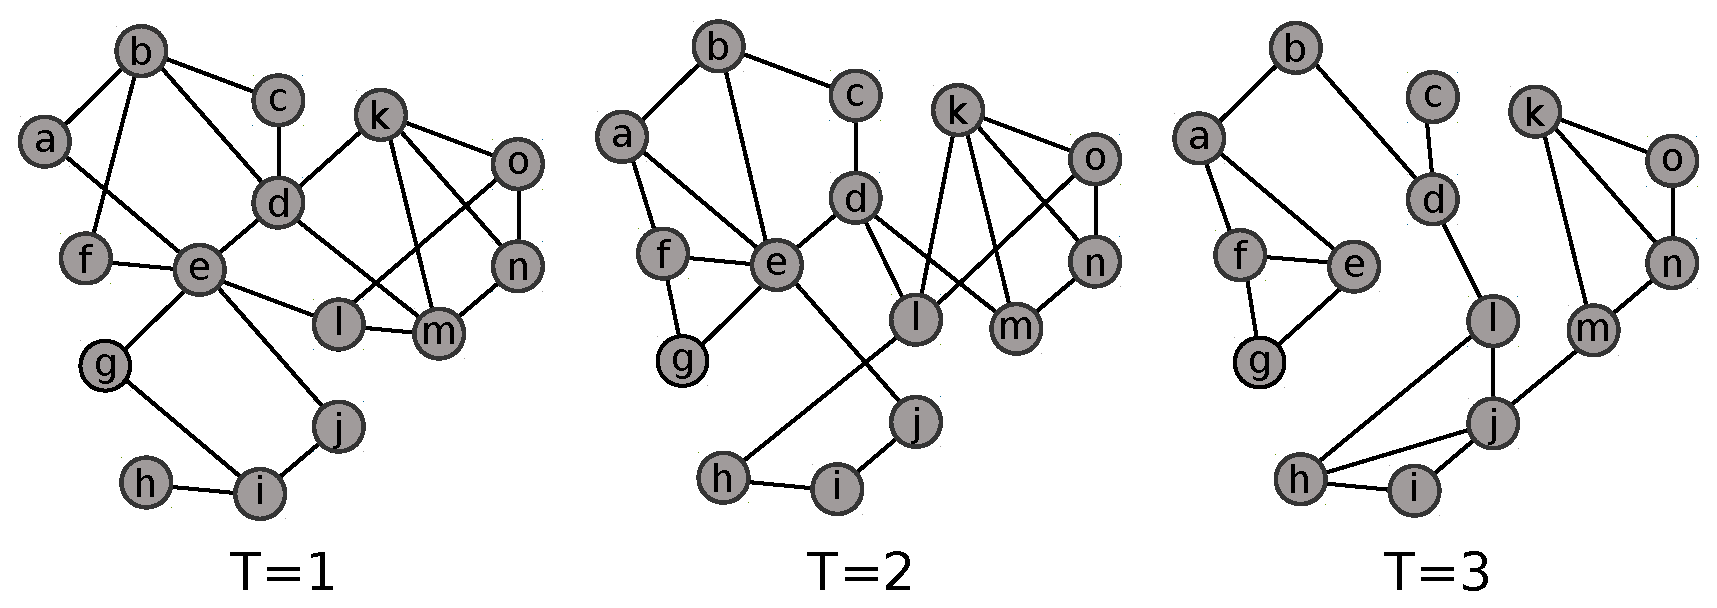
\includegraphics[width=0.8\linewidth]{img/Intro/TVG.eps}
\caption{Exemple de série de graphes sur trois intervalles de temps.}
\label{fig:exemple_TVG}
\end{figure}
La première solution qui a été apportée ne prend le temps en compte que partiellement.
Il s'agit de manipuler une série de graphes dont chaque graphe représente le réseau durant un intervalle de temps donné.
Ainsi, il est possible d'appliquer les outils de la théorie des graphes sur chaque intervalle.
Cependant chaque intervalle de temps est représenté par un graphe agrégé.
Il y a donc toujours une perte d'information.
Plus formellement, une série de graphe est définie par $\mathcal{G}=\{G_i\}_{i < T}$ où $T$ est un entier, voir la figure~\ref{fig:exemple_TVG}.

Cette définition initiale laisse le choix de la découpe du temps en intervalle.
Il est possible de choisir des intervalles de tailles égales ou non et disjoints ou chevauchants~\cite{Wang2012}.
Utiliser des intervalles à durée variable permet de mieux tenir compte de la dynamique.
Par exemple lors de l'étude d'interactions de personnes, il est très courant d'observer une très faible activité la nuit et une plus forte la journée.
Un graphe agrégeant ce qui se passe sur un intervalle de 5h sera vide dans le premier cas et peut être trop dense dans le second.
La détection d'intervalles pertinents est donc un vaste sujet de recherche~\cite{Rosvall2010,Krings2012,Ribeiro2013,Caceres2013,Peel2015,de2016detection}.

La notion même de temps est importante.
Albano \emph{et al.}~\cite{Albano2014} proposent d'utiliser une autre mesure qu'une unité temporelle, à savoir le nombre de changements comme mesure du temps.
Ainsi, le temps n'avance pas si aucun changement n'a lieu et au contraire il avance beaucoup si énormément de changements se produisent.
Cette notion de temps se rapproche de celle de Lamport~\cite{Lamport1978} dans ses travaux sur les systèmes distribués.

\paragraph{Détection de communautés}
Dans ce contexte de série de graphes, il y a eu assez tôt des méthodes de détection de communautés~\cite{Hopcroft2004,Sun2007,Lin2008,Asur2009}.
Il est, en effet, assez naturel d'appliquer une méthode de détection statique sur chaque graphe puis d'essayer de faire du suivi de communautés.
Le suivi de communautés consiste à comprendre comment une communauté donnée évolue, étant donné une série de graphes et une série de partitions.
Palla \emph{et al.}~\cite{Palla2007} ont été parmi les premiers à décrire les évolutions possibles d'une communauté.
Muni d'indicateurs de similarité tels que l'indice de Jaccard (voir la section~\ref{def:graphe_comparaison}) il est possible de trouver les communautés les plus proches aux instants précédant et suivant.
\`A partir de ces informations, six types d'évolutions d'une communauté sont définis:
\begin{description}
\item[Naissance] Une nouvelle communauté apparaît;
\item[Agrandissement] La communauté continue d'exister et s'agrandit;
\item[Fusion] Deux communautés fusionnent pour donner lieu à une nouvelle communauté;
\item[Division] Une communauté se sépare en deux nouvelles communautés à l'étape suivante;
\item[Rétrécissement] La communauté continue d'exister mais perd quelques n\oe{}uds;
\item[Mort] Une communauté cesse d'exister dans les graphes suivants.
\end{description}

Ce type de méthodes souffre de l'instabilité des méthodes de détection~\cite{Aynaud2010,Harenberg2014a}.
Si les partitions changent complètement entre deux graphes consécutifs, alors il est difficile de faire un réel suivi de communautés.
C'est pourquoi des méthodes essayent de forcer une certaine stabilité de la partition en ajoutant un coût de transition~\cite{Chakrabarti2006,Chen2013,Kalavathi2015}.
Une approche détournée pour garder une certaine stabilité est d'utiliser la partition trouvée précédemment comme base de recherche pour l'intervalle suivant~\cite{Aynaud2010,Lancichinetti2011a}.

Des extensions du SBM ont également été proposées par différents auteurs dans le cadre des séries de graphes.
Yang \emph{et al.}~\cite{Yang2011} sont parmi les premiers à considérer s'y attacher.
Ils considèrent que la probabilité d'un lien entre deux communautés est fixe et que ce qui change est l'affiliation des n\oe{}uds au cours du temps.
Ce processus de changement de communauté suit alors une chaîne de Markov cachée.
\`A l'inverse, Corneli \emph{et al.}~\cite{Corneli2016} considèrent une partition de n\oe{}uds fixe tout au long du temps et c'est l'activité entre deux communautés qui change selon l'intervalle de temps.
Xu et Hero~\cite{Xu2014} permettent à l'affiliation et à l'activité entre deux communautés de changer selon l'intervalle de temps.
Cependant, il semblerait que cette relaxation se fasse au dépens de l'identifiabilité des paramètres d'après Matias et Miele~\cite{Matias2015}.
Ils ont donc proposé une nouvelle méthode afin de résoudre ce problème.
De plus, cette méthode permet, de plus, de traiter des séries de graphes pondérés.

\subsubsection{Tenseurs 3D}
Il est possible de voir un graphe comme une matrice carrée d'adjacence.
Il en découle la conception d'une série de graphes comme un tenseur appartenant à $\mathcal{R}_{nnT}$.
Ce changement de point de vue permet l'application de méthodes d'algèbre linéaire, notamment la décomposition de tenseur.
C'est la méthode proposée par Gauvin \emph{et al.}~\cite{Gauvin2014} pour étudier la structure communautaire des interactions d'élèves.
Cependant ce genre de décomposition semble moins expressive que les SBM.


\subsubsection{Graphes multicouches}
\begin{figure}[h]
\centering
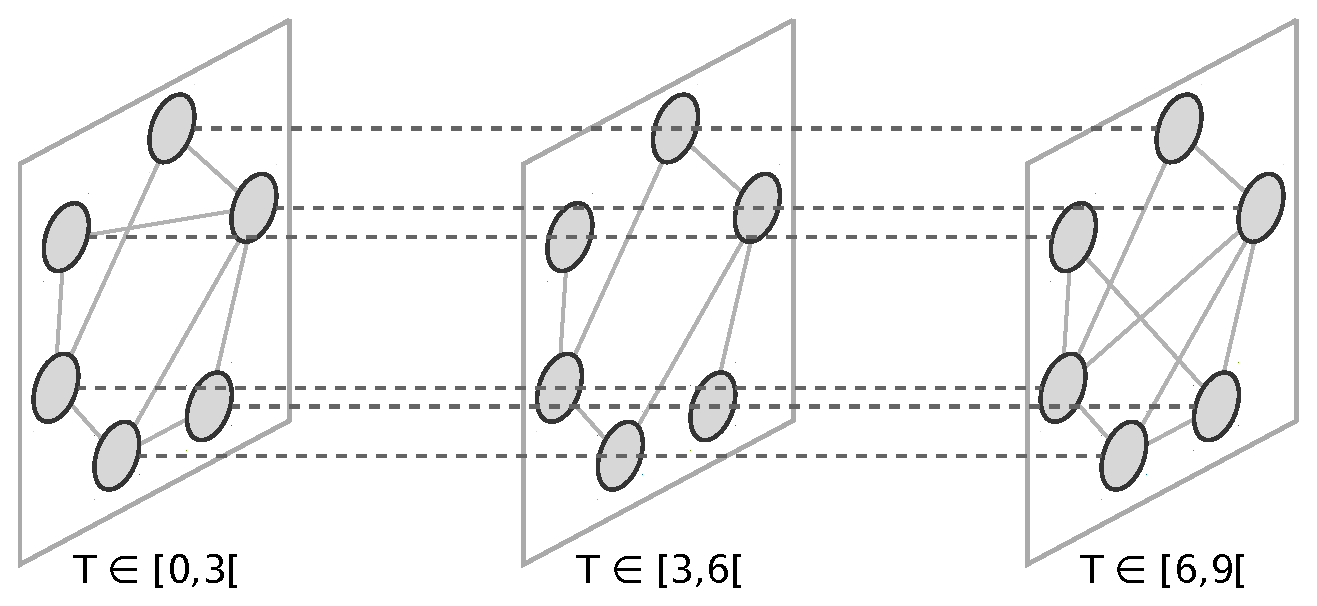
\includegraphics[width=0.7\linewidth]{img/Intro/multiplex.eps}
\caption{Graphe multicouches avec trois couches représentant le temps.
Les liens pleins (resp. pointillés) sont les liens intra-couches (resp. inter-couches).}
\label{fig:exemple_multiplex}
\end{figure}
La construction de graphes multicouches (\emph{multilayer} ou \emph{multiplex}) est proche de l'idée des séries de graphes.
Tout comme les séries de graphes, des n\oe{}uds et des liens sont créés à chaque intervalle pour représenter ce qui s'est déroulé durant l'intervalle de temps.
Cependant, le graphe multicouches ajoute des liens entre les n\oe{}uds de deux intervalles, voir l'illustration~\ref{fig:exemple_multiplex}.
Par conséquent, un graphe multicouches est un graphe où il existe deux types de liens, les liens intra-couches et les inter-couches et il existe $T$ répliques d'un même n\oe{}ud, une par intervalle de temps.
Les liens intra-couches représentent un connexion entre deux n\oe{}uds durant un intervalle de temps.
Les liens inter-couches représentent un lien entre deux n\oe{}uds sur deux intervalles différents.
Ces derniers sont utilisés pour identifier un même n\oe{}ud sur plusieurs intervalles et sont en général limités à relier deux couches consécutives.
En jouant sur les pondérations des liens intra- et inter-couches, il est possible de faire varier l'importance du temps.

Les graphes multicouches représentent les données évoluant dans le temps mais ils modélisent aussi très bien d'autres situations.
Par exemple, ils représentent facilement les différents moyens de transport dans une ville où chaque moyen de transport (bus, voiture, métro ...) est représenté par une couche.
Plusieurs travaux~\cite{DeDomenico2013,Kivela2014,Boccaletti2014,wehmuth2015multiaspect} décrivent les graphes multicouches et leurs applications.



\paragraph{Détection de communautés}
Grâce au formalisme de graphe multicouches, il est possible de traiter le temps de manière un peu plus fine que dans les séries de graphes car il permet de mieux suivre l'évolution des n\oe{}uds.
Comme un graphe multicouches est un graphe, il est possible d'adapter les méthodes existantes pour tenir compte des différents types de liens.
C'est le cas d'Infomap~\cite{de2015identifying}, de la modularité~\cite{Mucha2010,Bassett2013,Bazzi2016} et du SBM~\cite{Stanley,Peixoto2015c}.


\resume{
Les séries de graphes, les tenseurs 3D et les graphes multicouches permettent de prendre en compte le temps tout en autorisant l'utilisation de méthodes conçues pour des graphes statiques.
Or, ces approches reposent sur une découpe du temps en sous-intervalles durant lesquels le temps n'est plus pris en compte.
Il peut être délicat de définir ces intervalles de temps: la construction des graphes agrégés entraîne une perte d'information temporelle et cela a une influence sur la précision temporelle des structures communautaires qui sont manipulables.
Il n'est pas envisageable d'augmenter le nombre d'intervalles de temps car, d'une part, des graphes agrégés auraient très peu de liens et, d'autre part, le temps de calcul serait très fortement augmenté.
}

\subsection{Extensions sans perte d'information temporelle}
\label{subsec:pasperte_info}
\subsubsection{Graphes temporels}
\begin{figure}[h]
\centering
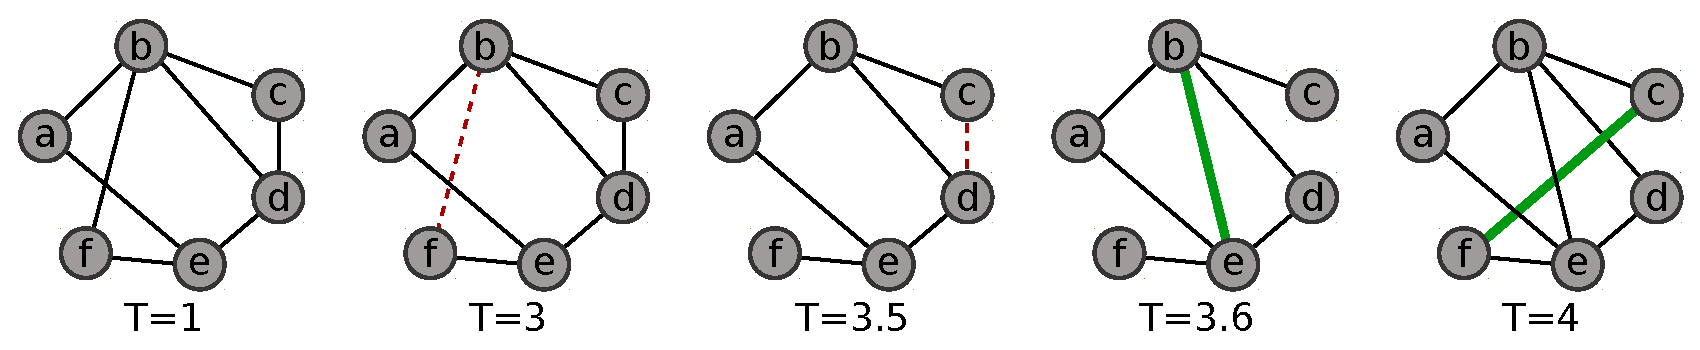
\includegraphics[width=0.9\linewidth]{img/Intro/evolvingGraph.eps}
\caption{Graphe temporel avec des ajouts de lien représentés en traits épais verts et des suppressions de lien représentées par des liens pointillés rouges.
}
\label{fig:exemple_evolving}
\end{figure}
Les graphes temporels (\emph{Time Varying Graph} ou \emph{Evolving Graph})
permettent de tenir compte de l'ensemble de l'information temporelle.
Pour cela au lieu de considérer des intervalles de temps, ils considèrent l'ensemble des modifications qui affectent le graphe: les ajouts et retraits de liens.
En pratique, cela revient à considérer sur chaque lien une fonction de présence dépendant du temps qui vaut $1$ à un instant $t$ si le lien existe à cet instant et $0$ sinon.
Ainsi, il est possible de connaître la structure de graphe à chaque instant.
Ce formalisme est présenté dans différents travaux~\cite{Casteigts2011,Wehmuth2015} et illustré dans la figure~\ref{fig:exemple_evolving}.
Dans cette figure, on voit apparaître l'ordre de modification du graphe.
Tout d'abord, les liens $(b,f)$ et $(c,d)$ disparaissent puis les liens $(b,e)$ et $(f,c)$ apparaissent chacun leur tour. 

\paragraph{Détection de communautés}
Dans un graphe temporel, une structure de graphe existe à chaque instant.
Il est donc possible de calculer après chaque modification l'évolution d'une métrique.
Par exemple, il est possible de calculer après l'ajout d'un lien le nouveau degré interne des n\oe{}uds concernés par ce changement.
En fonction de l'évolution de cette métrique, on décide alors d'ajouter ou de retirer un n\oe{}ud voire de fusionner deux communautés.
Li \emph{et al.}~\cite{Li2012a} se basent sur le nombre de liens que partage un n\oe{}ud avec les communautés environnantes.
Ainsi, un n\oe{}ud est toujours dans la communauté avec laquelle il partage le plus de liens.
Shang \emph{et al.}~\cite{Shang2014a}, Cordeiro \emph{et al.}~\cite{Cordeiro2016} et Sun \emph{et al.}~\cite{Sun2014} se basent sur l'évolution de la modularité.
Cependant, ces approches ne permettent pas de représenter l'ensemble des évolutions de communauté possibles, en particulier l'apparition d'une nouvelle communauté.
C'est pourquoi l'évolution de la structure courante peut mener à une structure ayant une faible qualité.
Une autre approche a été proposée par Cazabet \emph{et al.}~\cite{Cazabet2010} afin d'améliorer l'évolution de la partition.
Ils utilisent une métrique locale basée sur le nombre de chemins de longueur $2$ existant entre un n\oe{}ud et une communauté.
Après chaque modification, ils considèrent également la possibilité de créer une nouvelle communauté sous la forme d'une petite clique.
Ainsi, ils assurent une meilleure qualité de la partition au cours de l'évolution.


\subsubsection{Flots de liens}
\begin{figure}[h]
\centering
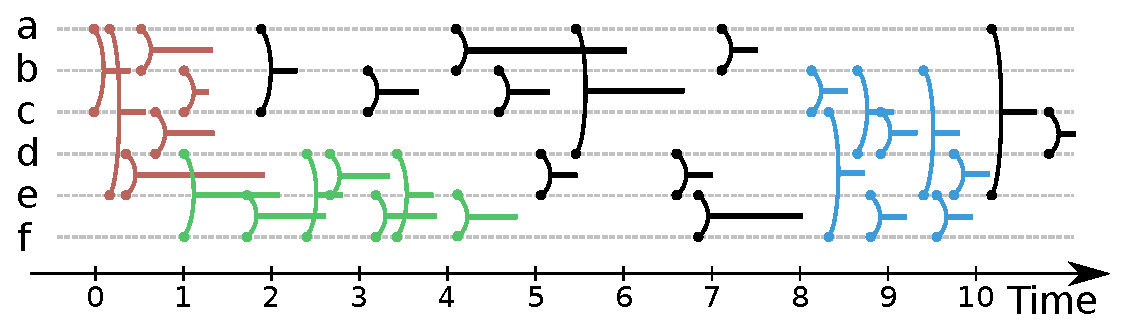
\includegraphics[width=0.9\linewidth]{img/Intro/Flot_de_liens.eps}
\caption{Flot de liens entre $6$ n\oe{}uds ( en ordonnées) au cours du temps (en abscisses).
Dans l'exemple, il existe un lien entre $a$ et $b$ durant l'intervalle $[4,6]$.
}
\label{fig:exemple_Flot_de_liens}
\end{figure}
Dans les graphes temporels, toute l'information temporelle est gardée.
Cependant, l'intuition derrière cette méthode est qu'il existe une structure de graphe à chaque instant.
Cette hypothèse n'est pas toujours vérifiée, en particulier lorsque les liens apparaissent et disparaissent très rapidement.
C'est le cas des appels téléphoniques qui durent rarement plus d'une heure ou bien de manière plus frappante avec les SMS et les courriels qui n'ont même pas de durée.
Dans ces contextes, il n'est pas possible de supposer qu'à chaque instant une structure de graphe pertinente existe.

Il faut donc un formalisme et des métriques qui s'adaptent à ce contexte.
C'est pour répondre à ce besoin que le formalisme de flot de liens a été pensé.
Le but est de construire un objet ne présupposant aucune structure et qui stocke toute l'information disponible.
Même si le formalisme ne présuppose aucune contrainte structurelle, il se peut que le réseau représenté en ait.
Par exemple dans les télécommunications, une personne ne peut appeler qu'une ou deux personnes en même temps.
Plusieurs travaux~\cite{Holme2013a,Holme2015b,Holme2015e} présentent des méthodes existantes pour étudier les flots de liens (également appelés \emph{temporal networks}) mais il n'existe, à notre connaissance, qu'un seul travail donnant un fondement théorique solide aux flots de liens.
Il s'agit de Batagel et Praprotnik~\cite{Batagelj2016} qui se basent sur l'algèbre.
Malheureusement avec une formulation purement algébrique, il semble difficile de transcrire l'ensemble des notions de graphes pour l'instant.
\bigskip

Prenons l'exemple des appels téléphoniques modélisable par un ensemble de quadruplets.
Un appel est représenté par un quadruplet $(b,e,u,v)$ où $b$ (resp. $e$) est le début (resp. la fin) de l'appel et $u$ et $v$ représentent des personnes en contact.
De cette manière, aucune information n'est perdue et, en ce sens, flots de liens et graphes temporels sont équivalents. 
Cependant, ce changement de perspective induit une réflexion différente selon le formalisme considéré.

Les différences dans les méthodes de représentation des graphes temporels de la figure~\ref{fig:exemple_evolving} et celle des flots de liens de la figure~\ref{fig:exemple_Flot_de_liens} illustrent bien ce changement de perspective, bien que les deux figures ne représentent pas le même réseau.
Dans l'exemple de la figure~\ref{fig:exemple_Flot_de_liens}, les n\oe{}uds sont représentés sur l'axe des ordonnées et le temps sur l'axe des abscisses.
Un lien dans cette visualisation est représenté par un arc vertical reliant deux n\oe{}uds et un trait horizontal représentant la durée du lien.
Ainsi dans l'exemple, il existe un lien entre les n\oe{}uds $a$ et $b$ dans l'intervalle $[4,6]$.

Dans un graphe temporel, on abordera plus souvent les questions d'évolution de communautés de n\oe{}uds ou de l'importance d'un n\oe{}ud.
Dans un flot de liens, on s'intéressera plus souvent au temps nécessaire pour que deux n\oe{}uds soient de nouveau en contact ou à l'importance d'un lien.
De manière très manichéenne et inexacte, le formalisme de graphe temporel pousse à étudier les relations et leur évolution alors que celui de flot de liens mets plus l'accent sur les interactions et leur dynamique.

\bigskip



Avec ce formalisme, la majorité des travaux sont seulement descriptifs car la structure n'a jamais été étudiée dans ce type d'objet.
De nombreux travaux ont étudié le temps séparant l'apparition de deux liens pour un n\oe{}ud~\cite{Malmgren2008,Malmgren2009}.
Il semblerait que ces temps inter-contacts soient très hétérogènes et que de nombreuses connexions apparaissent dans un faible intervalle de temps suivie de longues durées sans activité.
On parle alors de temps inter-contact \emph{bursty}.
Les effets des temps inter-contacts sur les phénomènes de contagions et de marches aléatoires sont très étudiés~\cite{Karsai2011,Karsai2012a,Starnini2012b,Rocha2013}.
Il n'y a cependant pas de conclusion définitive sur le sujet car la diffusion peut être accélérée ou ralentie par les temps inter-contacts selon la structure sous-jacente.

Il existe également quelques travaux qui s'intéressent plus à la structure des flots de liens, notamment à la présence de motifs~\cite{Kovanen2011a,Kovanen2013a}.
Dans un graphe, un motif est un petit sous-graphe, comme le triangle, qui est l'un des motifs les plus étudiés.
Dans les flots de liens, le temps est également pris en compte dans les motifs.
Il y a donc plusieurs variantes temporelles d'un même motif dans un graphe.
Prenons l'exemple d'un chemin entre quatre n\oe{}uds $A$, $B$, $C$ et $D$ qui est représenté dans le graphe par $\{(A,B), (B,C), (C,D)\}$.
Dans un flot de liens, il existe au moins deux variantes à ce motif soit
$\{(t_1,A,B), (t_2,B,C), (t_3,C,D)\}$ soit $\{(t_1,A,B), (t_2,C,D), (t_3,B,C)\}$ avec $t_1<t_2<t_3$.
Dans un cas, une information peut être propagée au fur et à mesure de $A$ vers $D$ tandis que dans l'autre ce n'est pas possible.
L'étude de la fréquence d'apparition de ces motifs dans le cas temporel permet d'observer si le flot de liens a une structure particulière. 



\paragraph{Détection de structures}
Il existe peu de méthodes détectant des structures décrivant l'ensemble d'un flot de liens.
Rozenshtein \emph{et al.}~\cite{rozenshtein2014} se penchent sur la détection de la zone la plus dense dans les flots de liens.
Ils permettent de capturer un ensemble de n\oe{}uds et plusieurs intervalles de temps disjoints tels que ces n\oe{}uds sur ces intervalles aient le degré moyen le plus élevé dans le graphe agrégé sur ces intervalles.
Bien que la mesure utilisée ne tienne pas directement compte du temps, la méthode permet de mettre en évidence une partie du flot de liens.

Il existe également des travaux conduits au sein de l'équipe~\cite{Viard2016,viard:hal-01208330} sur la notion de cliques dans les flots de liens sans durée, c'est à dire un ensemble de $(b,b,u,v)$.
Ils généralisent la notion de clique à ces flots de liens: pour un delta donné, une delta-clique est un ensemble de n\oe{}uds et un intervalle de temps, tels que toutes les paires de n\oe{}uds dans cet ensemble interagissent au moins tous les delta sur cet intervalle.
Dans ce cadre, un premier algorithme permettant d’énumérer les delta-cliques a été proposé.
Cet algorithme a, de plus, été appliqué avec succès sur différents jeux de données.



Une méthode de type SBM a été proposée par Matias \emph{et al.}~\cite{Matias2015a}.
Elle est très proche de celle proposée par Corneli \emph{et al.}~\cite{Corneli2016}, citée précédemment.
En effet, l'affiliation des n\oe{}uds est fixe et c'est l'activité d'une communauté qui change au cours du temps.
La grosse différence ici est que l'activité varie de manière continue dans le temps.
Ainsi l'apparition d'un lien dépend de la réalisation d'un processus de Poisson non homogène qui change selon les communautés.
Cependant, leur méthode ne permet pas de considérer les changements de communauté.



% centralité \cite{,Kim2012, Pfitzner2013a,Praprotnik2015,Scholtes2015,Costa2015,Takaguchi2016}

\resume{
Les graphes temporels et les flots de liens ne souffrent pas d'agrégation temporelle.
Ils ont donc un pouvoir expressif plus important que les formalismes présentés précédemment.
Formellement, flots de liens et graphes temporels sont équivalent dans le sens où un graphe temporel peut être représenté en un flot de liens et \emph{vice versa}.
En revanche, ils diffèrent dans le point de vue considéré.
Dans un graphe temporel, on suppose en général qu'il existe une structure de graphe représentant le réseau à chaque instant et les métriques de graphes sont pertinentes.
Dans un flot de liens, il n'existe en général pas de structure pertinente à un instant donné et par conséquent les métriques de graphes ne sont pas pertinentes.
Cette différence implique d'utiliser des mesures différentes et, en particulier, de créer de nouvelles métriques pour les flots de liens.
Cela explique notamment pourquoi il n'existe pour l'instant qu'assez peu de travaux traitant de la structure des flots de liens.
Cette différence de perspective entraîne également un déplacement du centre d'intérêt.
Dans les graphes temporels, on aura plutôt tendance à étudier les relations et leur évolution.
\`A l'inverse, on s'intéresse plutôt aux interactions et leur répartition dans les flots de liens.
Ainsi, les deux formalismes coexistent et répondent à des besoins différents.}

\section{Bilan}

Pour les graphes statiques, il existe de très nombreuses méthodes capturant une structure des n\oe{}uds soit via une partition soit via une couverture.
L'abondance de méthodes existantes s'explique par la diversité des définitions de communautés existantes.
Les structures capturées permettent de mieux comprendre l'organisation du graphe mais aussi de mieux comprendre le type d'un n\oe{}ud.


Avec l'émergence de nouvelles données incorporant l'information temporelle, il est pertinent d'adapter la théorie des graphes pour prendre en compte le temps.
L'extension temporelle des graphes est un champ de recherche très récent et de nombreuses méthodes de détection de communautés dans ce contexte vont voir le jour.
Cependant, tous les formalismes existants ne sont pas équivalents et ils limitent parfois les solutions possibles.


Il y a d'une part les formalismes se rapprochant de la théorie des graphes: séries de graphes, tenseurs 3D et graphes multicouches.
Ces formalismes sont proches des graphes statiques et il est même possible d'y appliquer des méthodes statiques.
En revanche, la prise en compte du temps n'est que partielle.
Il y a toujours une forme d'agrégation temporelle et il n'est pas possible d'avoir une vision très fine de l'objet d'étude.
De plus, les solutions existantes reposent sur le suivi de communautés qui ne semble pas être un problème résolu.


D'autre part, les formalismes de graphes temporels et de flots de liens capturent toute l'information temporelle.
Ils ne souffrent donc pas de perte d'information.
Ces deux formalismes, bien qu'équivalents, ne présupposent pas la même structure sur les données sous-jacentes.
Dans un graphe temporel, les liens durent assez longtemps et par conséquent il existe une structure de graphe pertinente à chaque instant.
Dans les flots de liens, les liens sont plus courts et il n'existe aucune structure de graphe à un instant donné.
Par conséquent, ces deux formalismes répondent à des situations différentes.
Par exemple, les études des temps inter-contacts sont très majoritairement conduites en utilisant le formalisme de flot de liens.
Il semble donc plus aisé d'utiliser un flot de liens qu'un graphe temporel lorsque l'on souhaite étudier la structure des interactions.



Au cours de cette thèse, nous nous intéressons à la structure communautaire que peuvent former les liens dans le temps.
Nous ne pouvons utiliser, ni les formalismes basés sur une agrégation temporelle à cause de la perte d'information, ni le formalisme de graphe temporel car ils considèrent des situations assez différentes de celles que nous étudions.
C'est pourquoi le formalisme de flot de liens semble être le plus adapté pour étudier la structure des liens.
Il n'existe que peu de travaux définissant formellement les flots de liens et traitant de leur structure.
C'est pourquoi dans le chapitre~\ref{chap:def_flot}, nous définissons plus formellement ce qu'est un flot de liens ainsi que les métriques utilisées tout au long de cette thèse.
Nous présentons dans les chapitres suivants nos travaux sur les structures de liens.


